\documentclass[12pt,oneside]{reedthesis}

\usepackage{graphicx,latexsym}
\usepackage{amsmath}
\usepackage{amssymb,amsthm}
\usepackage{longtable,booktabs,setspace}
\usepackage[hyphens]{url}
\usepackage{hyperref}
\hypersetup{breaklinks=true,
            bookmarks=true,
            pdfauthor={Erik Gahner Larsen and Zoltán Fazekas},
            pdftitle={Quantitative Politics with R},
            colorlinks=true,
            citecolor=blue,
            urlcolor=blue,
            linkcolor=blue,
            pdfborder={0 0 0}}
\urlstyle{same}
\usepackage{lmodern}
\usepackage{float}
\floatplacement{figure}{H}

\usepackage{rotating}

\usepackage[hmargin=3cm,vmargin=2.5cm]{geometry}
\usepackage[utf8]{inputenc}
\usepackage[T1]{fontenc}
\usepackage{multirow}
\usepackage{booktabs}
\usepackage{microtype}
\usepackage{nag}
\usepackage{cleveref}
\usepackage{float}
\usepackage{dcolumn}
\usepackage{pdflscape}
\usepackage{multirow}
\usepackage{caption}
\usepackage{footmisc}
\usepackage{pdflscape}
\usepackage{array}
\usepackage{cleveref}
\usepackage{longtable}

\renewcommand{\hyperref}[2][???]{\autoref{#1}}
\def\chapterautorefname{Chapter}
\def\sectionautorefname{Section}
\def\subsectionautorefname{Subsection}

\usepackage{caption}
\captionsetup{width=5in}

\title{\Huge{ Quantitative Politics with R } \vspace{2em}}
\author{Erik Gahner Larsen and Zoltán Fazekas}
\date{Februar 06, 2018}

\renewcommand{\contentsname}{Table of Contents}

\setlength{\parskip}{0pt}

% Added by CII

\providecommand{\tightlist}{%
  \setlength{\itemsep}{0pt}\setlength{\parskip}{0pt}}


% End of CII addition
%%
%% End Preamble
%%
%

%\usepackage{MinionPro}
\linespread{1.3}

\usepackage{amsthm}
\newtheorem{theorem}{Theorem}[section]
\newtheorem{lemma}{Lemma}[section]
\theoremstyle{definition}
\newtheorem{definition}{Definition}[section]
\newtheorem{corollary}{Corollary}[section]
\newtheorem{proposition}{Proposition}[section]
\theoremstyle{definition}
\newtheorem{example}{Example}[section]
\theoremstyle{definition}
\newtheorem{exercise}{Exercise}[section]
\theoremstyle{remark}
\newtheorem*{remark}{Remark}
\newtheorem*{solution}{Solution}
\begin{document}

% Everything below added by CII
      \maketitle
  
  \frontmatter % this stuff will be roman-numbered
  \pagestyle{empty} % this removes page numbers from the frontmatter

  
  
      \hypersetup{linkcolor=black}
    \setcounter{tocdepth}{2}
    \tableofcontents
  
  
  
  
  
  \mainmatter % here the regular arabic numbering starts
  \pagestyle{fancyplain} % turns page numbering back on

  \chapter{Introduction}\label{introduction}
  
  If you want to conduct quantitative analyses of political phenomena,
  \texttt{R} is by far the best software you can use. Importantly, data
  analysis is no longer restricted to analyzing survey data, but does now
  include social media data, texts, images, geographic data (\emph{GIS}),
  and so forth.
  
  In this book, we aim to provide an easily accessible introduction to
  \texttt{R} for the study of different types of data. The book will teach
  you how to get different types of data into \texttt{R} and manipulate,
  analyze and visualize the data.
  
  Compared to other statistical softwares, such as Excel, SPSS, Stata and
  SAS, you will experience that \texttt{R} is completely different. First
  in a bad way: things are not as easy as they used to be. Then in a good
  way: once you learn how to do different tasks in \texttt{R}, you will be
  ashamed when you look back at the old you doing analyses in SPSS.
  
  In this chapter you will find an introduction to \texttt{R}. First, we
  ask the obvious and important question, why R? Second, we help you
  install what you need. Third, we introduce you to the basic logic of
  \texttt{R} so you are ready for the chapters to come.
  
  \section{\texorpdfstring{Why \texttt{R}?}{Why R?}}\label{why-r}
  
  First, \texttt{R} is an \emph{open source} statistical programming
  language. \texttt{R} is free, and while you might not pay for Stata or
  SPSS because you are a student, you will not have free access to this
  forever. This is not the case with \texttt{R}. On the contrary, you will
  \emph{never} have to pay for \texttt{R}.
  
  Second, \texttt{R} provides a series of opportunities you don't have in
  SPSS and Stata. \texttt{R} has an impressive package ecosystem on CRAN
  (the \textbf{c}omprehensive \textbf{R} \textbf{a}rchive
  \textbf{n}etwork) with more than 12,000 packages created by other users
  of \texttt{R}.
  
  Third, some of the most beautiful figures you will find today are
  created in \texttt{R}. Big media outlets such as The New York Times and
  FiveThirtyEight use \texttt{R} to create figures. In particular the
  package \texttt{ggplot2} is popular to create figures and we will work
  with this package below.
  
  Fourth, there is a great community of \texttt{R} users that are able to
  help you when you encounter a problem (which you undoubtly will).
  \texttt{R} is a very popular software and in great demand meaning that
  you will not be the first (nor the last) to experience specific issues
  in your data analysis. Accordingly, you will find a lot of help on
  Google and other places to a much greater extent than for other types of
  software.
  
  Fifth, while you can't do as much point-and-click as in SPSS and Stata,
  this approach facilitates that you can reproduce your work. When you are
  doing something i \texttt{R} with commands (in a script) is it easy to
  document. So, while you do not see a pedagogical graphical user
  interface in \texttt{R} with a limited set of buttons to click, this is
  more of an advantage than a limitation.
  
  \section{\texorpdfstring{Installing
  \texttt{R}}{Installing R}}\label{installing-r}
  
  To install the \texttt{R}, you will have to install 1) the \texttt{R}
  language and 2) RStudio, the graphical user interface. To install the
  \texttt{R} language, follow this procedure:
  \begin{enumerate}
  \def\labelenumi{\arabic{enumi}.}
  \tightlist
  \item
    Go to \url{https://cloud.r-project.org}.
  \item
    Click \emph{Download R for Windows} if you use Windows or
    \emph{Download R for (Mac) OS X} if you use Mac.
  \end{enumerate}
  If you use Windows:
  \begin{enumerate}
  \def\labelenumi{\arabic{enumi}.}
  \setcounter{enumi}{2}
  \tightlist
  \item
    Click on \emph{base}.
  \item
    Click the top link where you can download \texttt{R} for Windows.
  \item
    Follow the installation guide.
  \end{enumerate}
  If you use Mac:
  \begin{enumerate}
  \def\labelenumi{\arabic{enumi}.}
  \setcounter{enumi}{2}
  \tightlist
  \item
    Select the most recent \texttt{.pkg} file under \emph{Files:} that
    fits your OS X.
  \item
    Follow the installation guide.
  \end{enumerate}
  If you encounter problems with the installation guide, make sure that
  you did download the correct file \emph{and} that your computer meets
  the requirements. If you did this and still encounter problems, you
  should get an error message you can type into Google and find relevant
  information on what to do.
  
  You should now have the \texttt{R} language installed on your computer.
  
  \section{Installing RStudio}\label{installing-rstudio}
  
  RStudio is an integrated development environment (IDE) and makes it much
  easier to work in \texttt{R} compared to the standard (``base'') R. This
  is also available for free. To install RStudio, follow these steps:
  \begin{enumerate}
  \def\labelenumi{\arabic{enumi}.}
  \tightlist
  \item
    Go to:
    \url{https://www.rstudio.com/products/rstudio/download/\#download}.
  \item
    Click on the installer file for your platform, e.g.~Windows or Mac OS
    X.
  \item
    Follow the installation guide.
  \end{enumerate}
  You should now have RStudio installed on your computer. When you open
  \texttt{R} you will see a graphical interface as in Figure
  \ref{fig:interface}.
  \begin{figure}
  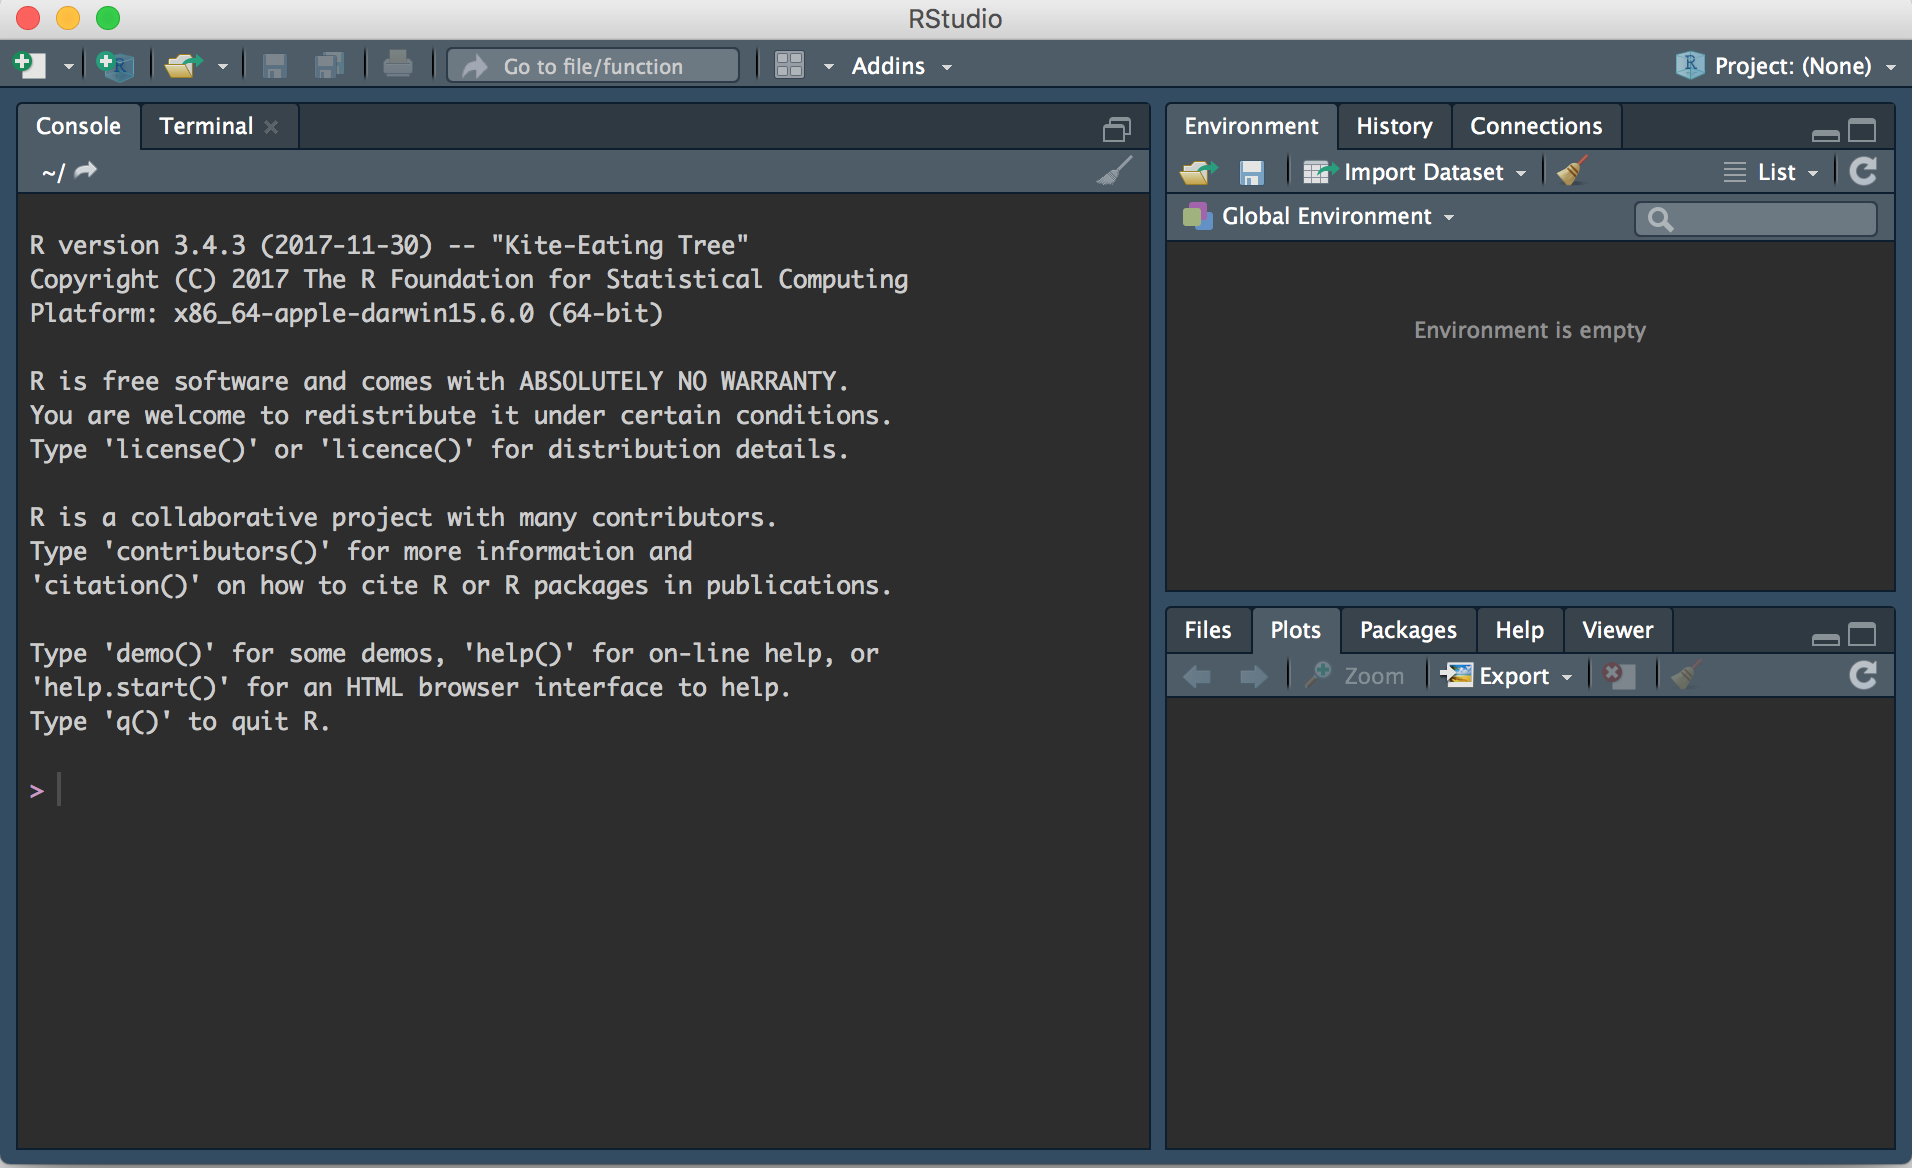
\includegraphics[width=1\linewidth]{fig/rstudio} \caption{Graphical interface in RStudio}\label{fig:interface}
  \end{figure}
  There are three different windows. However, one is missing, and that is
  the window where you will write most of your scripts. You can get this
  window by going to the top menu and select \texttt{File} \(\rightarrow\)
  \texttt{New\ File} \(\rightarrow\) \texttt{R\ Script}. This should give
  you four windows as shown in Figure \ref{fig:interfaceexplain}.
  \begin{figure}
  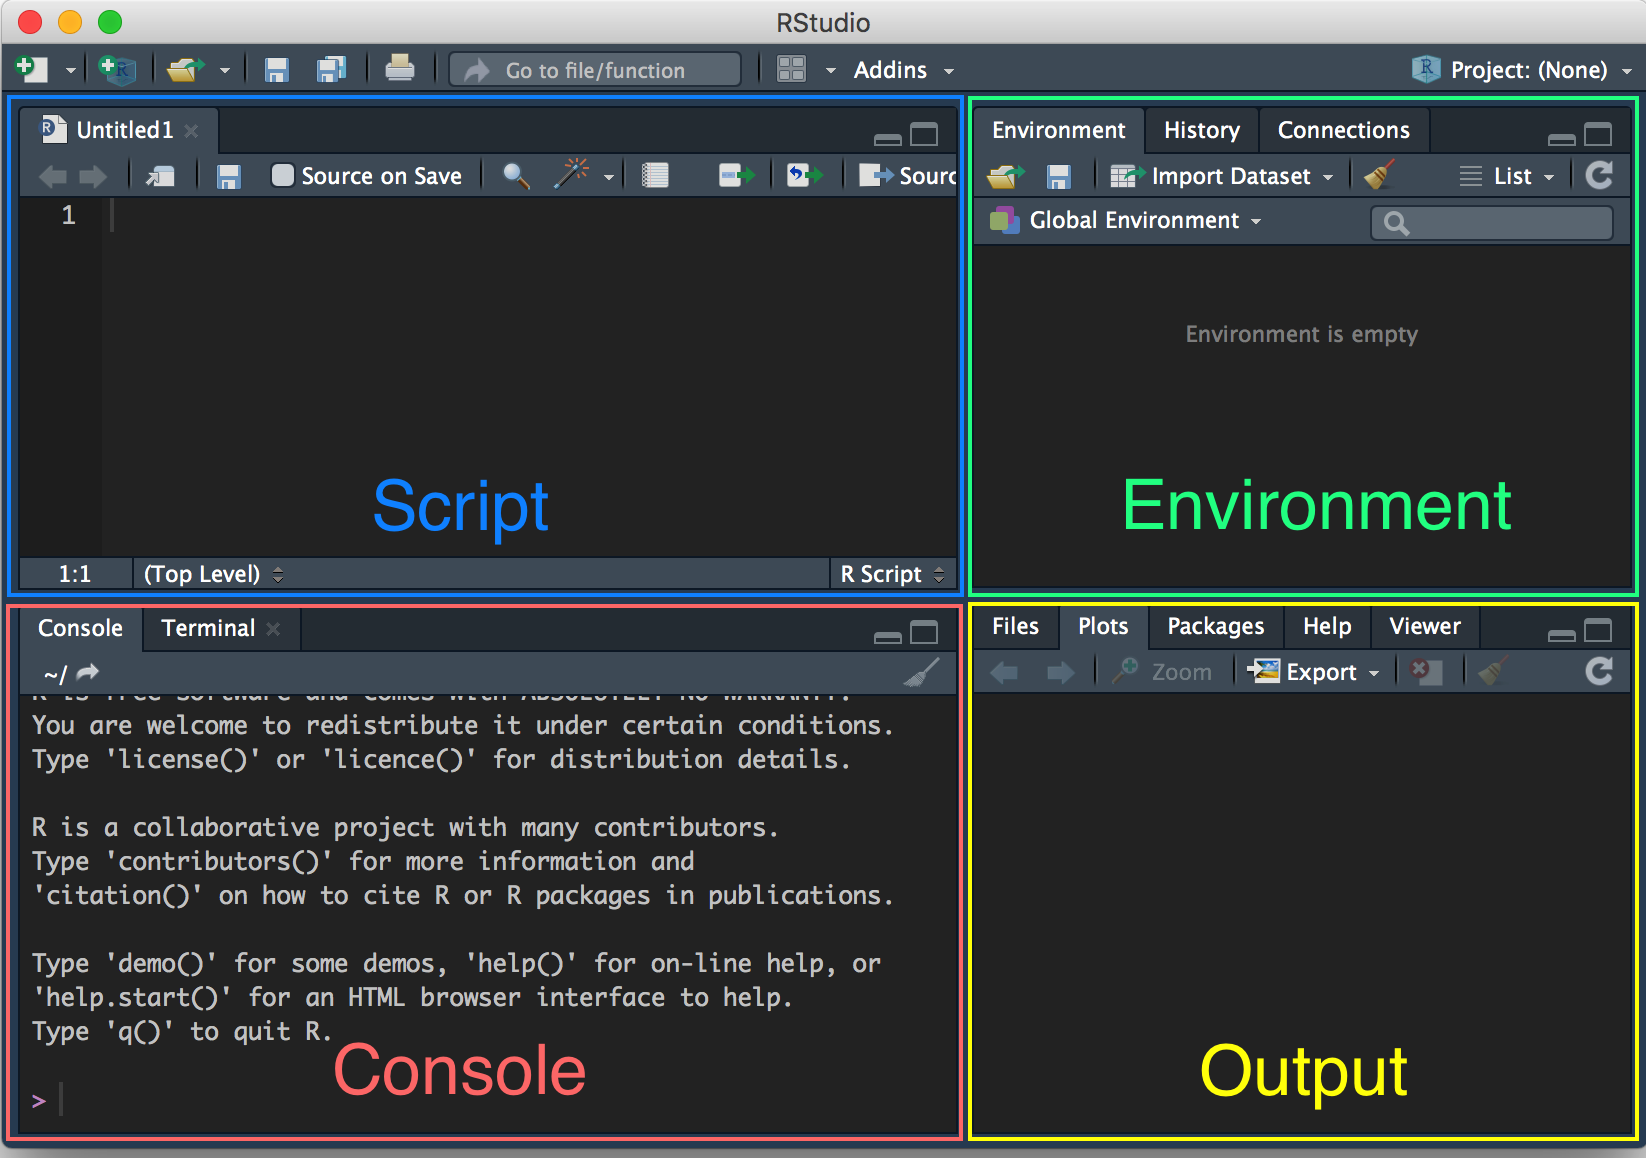
\includegraphics[width=1\linewidth]{fig/rstudio_env} \caption{Graphical interface in RStudio, explained}\label{fig:interfaceexplain}
  \end{figure}
  In the figure, we have emphasized the four windows: script, environment,
  output, and console. The \emph{script} is where you will have your
  \texttt{R} code and make changes. The \emph{environment} is where you
  can see what datasets, variables and other parts you have loaded into R.
  The \emph{output} is where you can see figures you create. The
  \emph{console} is where you can see some output and run commands.
  
  Everything you do in \texttt{R} can be written as commands. This ensures
  that you will always be able to document your work (in your script). In
  the console, you can see a prompt (\texttt{\textgreater{}}). Here, you
  can write what what you want \texttt{R} to do. Try to write \texttt{2+2}
  and hit \texttt{Enter}. This should look like this:
  \begin{Shaded}
  \begin{Highlighting}[]
  \DecValTok{2}\OperatorTok{+}\DecValTok{2}
  \end{Highlighting}
  \end{Shaded}
  \begin{verbatim}
  [1] 4
  \end{verbatim}
  The code you have entered in the console cannot be traced later.
  Accordingly, you will have to save the commands you want to keep in the
  script. Even better, you should write your commands in the script and
  ``run'' them from there. If you write \texttt{2+2} in the script, you
  can mark it and press \texttt{CTRL+R} (Windows) or \texttt{CMD+ENTER}
  (Mac). Then it will run the part of the script that is marked in the
  console. Insert the code below in your script and run it in the console:
  \begin{Shaded}
  \begin{Highlighting}[]
  \DecValTok{50}\OperatorTok{*}\DecValTok{149}
  \DecValTok{3}\OperatorTok{**}\DecValTok{2}        \CommentTok{# 3^2}
  \DecValTok{2}\OperatorTok{**}\DecValTok{3}        \CommentTok{# 2^3}
  \KeywordTok{sqrt}\NormalTok{(}\DecValTok{81}\NormalTok{)    }\CommentTok{# 81^0.5}
  \end{Highlighting}
  \end{Shaded}
  As you can see, we have used \texttt{\#} as well. The \texttt{\#} sign
  tells \texttt{R} that everything after that sign on that line shouldn't
  be read as code but as a comment. In other words, you can write comments
  in your script that will help you remember what you are doing - and help
  others understand the meaning of your script. For now, remember to
  document everything you do in your script.
  
  Notice also that we use a function in the bottom, namely
  \texttt{sqrt()}. A lot of what we will be doing in \texttt{R} is with
  functions. For example, to calculate a mean later we will use the
  \texttt{mean()} function. In the next section we will use functions to
  install and load packages.
  
  \section{\texorpdfstring{Installing \texttt{R}
  packages}{Installing R packages}}\label{installing-r-packages}
  
  We highlighted above that one of the key advantages of using \texttt{R}
  is the package system. In \texttt{R}, a package is a collection of data
  and functions that makes it easier for you do to what you want. The sky
  is the limit and the only thing you need to learn know is how to install
  and load packages.
  
  To install packages, you will have to use a function called
  \texttt{install.packages()}. We will install a package that installs a
  lot of the functions we will be using to manipulate and visualise data.
  More specifically, we will work within the tidyverse (you can read more
  at \href{http://tidyverse.org/}{tidyverse.org}). To intall this package
  type:
  \begin{Shaded}
  \begin{Highlighting}[]
  \KeywordTok{install.packages}\NormalTok{(}\StringTok{"tidyverse"}\NormalTok{)}
  \end{Highlighting}
  \end{Shaded}
  You only need to install the package once. In other words, when you have
  used \texttt{install.packages()} to install a packagae, you will not
  need to install that specific package again. Note that we put
  \texttt{tidyverse} in quotation marks. This is important when you
  install a package. If you forget this, you will get an error.
  
  While you only need to install a package once, you need to load the
  package every time you open \texttt{R}. This is a good thing as you
  don't want to have all your installed \texttt{R} packages working at the
  same time. For this reason, most scripts begin with loading the packages
  that is needed. To load a package, we use the function
  \texttt{library()}:
  \begin{Shaded}
  \begin{Highlighting}[]
  \KeywordTok{library}\NormalTok{(}\StringTok{"tidyverse"}\NormalTok{)}
  \end{Highlighting}
  \end{Shaded}
  To recap, it is always a good idea to begin your script with the
  package(s) you will be working with. If we want to have a script where
  we load the \texttt{tidyverse} package and have some of the commands we
  ran above, the script could look like the script presented in Figure
  \ref{fig:interfacescript}.
  \begin{figure}
  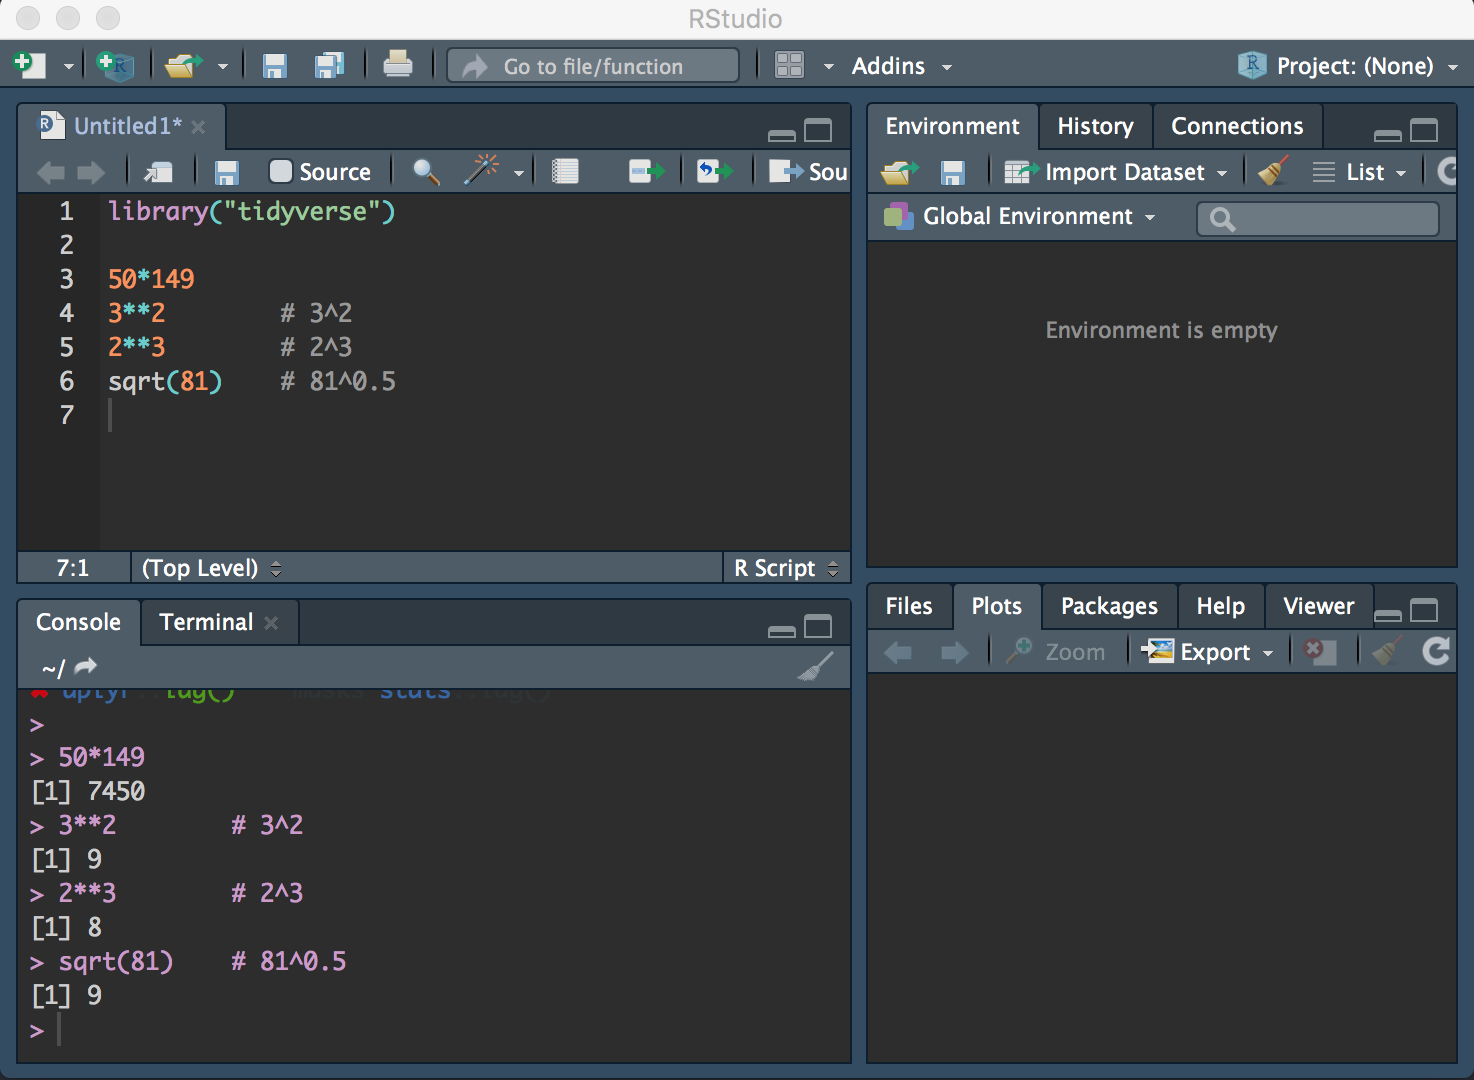
\includegraphics[width=1\linewidth]{fig/rstudio_script} \caption{A script in RStudio}\label{fig:interfacescript}
  \end{figure}
  If you want to save your script you can select \texttt{File}
  \(\rightarrow\) \texttt{Save}, where you can pick a destination for your
  script.
  
  \section{Errors and help}\label{errors-and-help}
  
  As noted above, you will encounter problems and issues when you do stuff
  in \texttt{R}. Sadly, there are many potential reasons to why your
  script might not be working. Your version of \texttt{R} or/and RStudio
  might be too old or too new, you might be using a function that has a
  mistake, you might not have the data in the right format etc.
  
  Consequently, we cannot provide a comprehensive list of errors you might
  get. The best thing to do is to learn how to find help online. Here, the
  best advice is to use Google and, when you search for help, always
  remember to mention R in your search string, and, if you are having
  problems with a specific package, also the name of the package.


  % Index?

\end{document}
